\section{Evaluation}
\label{sec:evaluation}

In this section, we analyze the performance of our algorithm
to check the equivalence of context-free session types. 
To do so, we have implemented the algorithm we have presented
thus far (sketched in Listings~\ref{lst:toGrammar}, 
\ref{lst:prune}, \ref{lst:algorithm}) 
in Haskell, and used Haskel compiler 
Glasgow Haskell Compiler, GHC version 8.6.3, from which we have 
obtained the running times we present throughout this section.
The machine used for the evaluation was a Mac mini at 3,6 GHz Intel 
Core i3 with 8 GB of memory. 

At this stage, we were aiming to analyze the performance of
our type equivalence checking algorithm, when we came across 
a particular test whose context-free session types where:
\begin{equation}
\label{ex:chaotic}
	\begin{aligned}
		S &\triangleq \mu x . \&\{ \mathsf{add}: x;x; !\,\intk,
							       \mathsf{const}: ?\,\intk;!\in\intk,
							       \mathsf{mult}: x;x;!\,\intk\}\\
		T &\triangleq \mu x . \&\{ \mathsf{add}: x;x,
							  	   \mathsf{const}: ?\,\intk,
							       \mathsf{mult}: x;x\}; !\,\intk
	\end{aligned}
\end{equation}
\lstinline{equivalent S T} took 4810.21 seconds to decide the equivalence
positively. This would not be a reasonable amount of time for a
feasible compiler. Hence, we started to pave the way to improve the
running times. For this purpose, we propose:
\begin{enumerate}
	\item to iterate the simplification stage until a fixed point
	on the \emph{simplest children nodes} is reached;
	\item to consider a double ended queue, where \emph{promising} 
	children nodes would be prepended, as opposed to enqueuing 
	all new nodes.
\end{enumerate}

If, in one hand, we believe that the computation of the expansion
tree can be speeded up by extending the simplification phase, on 
the other hand we believe that a double ended queue will allow us to 
prioritize nodes that potentially allow us to reach an empty node faster.
The latter is obtained by prepending nodes that are already empty or, 
either, whose pairs $(\vec X, \vec Y)$ are such that $|\vec X|\leq 1$
and $|\vec Y| \leq 1$.
For the former, we need to check that a fixed point exists and,
hence, for a given node $N$, we are able to compute the 
\emph{simplest} children nodes derived from $N$ using the
simplification rules.

\begin{theorem}
	\todo{fixed point exists}{}
\end{theorem}

We have tested the several combination of the previous proposals
in our algorithm on a batch of 138 tests. The results are presented 
in Figure~\ref{fig:results}.

\begin{figure}[h]
	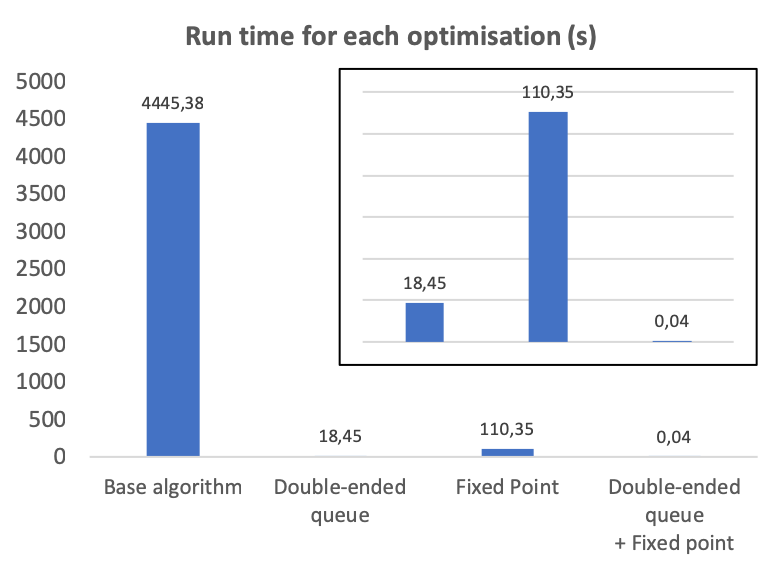
\includegraphics[height=4.8cm]{img/run_time}	\qquad 
	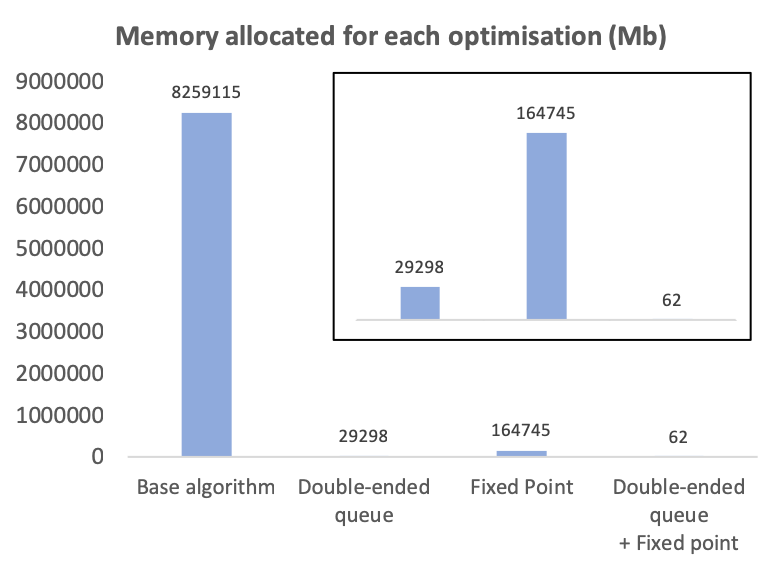
\includegraphics[height=4.8cm]{img/memory_alloc}	
	\caption{Test results: running times (on the left) and
	memory allocated (on the right) checking the equivalence 
	of context-free session types in 138 tests.}
	\label{fig:results}
\end{figure}

The running times and memory allocated presented in 
Figure~\ref{fig:results}, exhibit an improvement on more 
than 12000000\%. The decision for the equivalence of our particular
example in~\eqref{ex:chaotic} took now only 0.01
seconds. For this reasons, our proposal for an
algorithm to check the equivalence of context-free session types 
stands on adapting the simplification stage to enable double ended 
enqueueing and the computation of a fixed point at the
simplification phase. Listing~\ref{lst:enhanced} presents
an enhanced version of the simplification stage coping the new
proposals.
\begin{lstlisting}[caption={Haskell code for the adapted simplification
                   stage of the improved algorithm to check the 
                   equivalence of context-free session types},
                   label={lst:enhanced} ,captionpos=b] 
simplify :: Productions -> Ancestors ->  Node -> NodeQueue -> NodeQueue
simplify g a n q = foldr enqueueNode (Queue.dequeue q) m'
  where m' = findFixedPoint g (Set.singleton (n,a))

enqueueNode :: (Node,Ancestors) -> NodeQueue -> NodeQueue
enqueueNode (n,a) q
 | Set.null n           = Queue.priorityEnqueue (n,a) q
 | maximumLength n == 1 = Queue.priorityEnqueue (n,a) q
 | otherwise            = Queue.enqueue (n,a) q

findFixedPoint :: Productions -> Set.Set (Node,Ancestors) -> 
                  Set.Set (Node,Ancestors)
findFixedPoint g nas
  | nas == nas' = nas
  | otherwise = findFixedPoint g nas'
  where nas' = if allNormed p
                then foldr (apply p) nas [reflex,congruence,bpa2]
                else foldr (apply p) nas [reflex,congruence,bpa1,bpa2]
\end{lstlisting}


